% ##################################################################################################################
\section{Sochi}
\label{ch:scenarios:sochi}
\hfill \textbf{Author:} Marcel Rieser


Major sport events often attract a huge crowd of spectators and media
reporterts, they need many official helpers in various locations to guide and
support attendants, and---naturally---require all athletes to be in
the right place at the right time.  For large, international contests like
olympic games or soccer championships, accommodations are rarely close to the
event facilities, making it necessary to transport spectators, media, helpers
and athletes efficiently over large distances. As such events typically run for
multiple days or even weeks, with ever-changing combinations of locations and
times where actual competitions take place, a lot of planning is required to
ensure that all attendants can reach their event locations in time.

Masterconcept Consulting GmbH, an Austrian consulting company, has specialized
itself to provide high-level concepts for large sport events as mentioned above.  In a
move to better serve its clients, it developed ITSOS (Intermodal Transport
Simulation \& Operation System), a GIS-based system to support its transport
planners in the creation of mobility concepts for major events as well as for
regional planning.  ITSOS heavily depends on MATSim to simulate the planned
concepts in order to verify if the special infrastructure at major events is
capable to transport all the persons within a useful time to and from
their specific event locations.

Senozon was responsible to integrate MATSim with ITSOS and add ITSOS-specific
functionality to MATSim. Together, a test scenario was created, depicting the
olympic winter games 2014 in Sochi.



\subsection{System Overview}

ITSOS uses ESRI ArcGIS for storing and editing infrastructure data like road
and train networks and event facilities. In addition, a custom plugin provides a
graphical user interface inside ArcGIS to specify transit routes and schedules,
vehicle types and their assignments to lines and departures, as well as methods
to describe the expected travel demand. Transport planners can create and manage
scenarios and scenario-variants directly from the custom user interface
available inside ArcGIS.

After the successfull modelling of a scenario in ArcGIS, a planner can export
the network and transit schedule in MATSim's XML format directly from ITSOS to a
local directory. The travel demand information, consisting of activity-chains
with with zone- or facility-references and the number of persons having such a
chain, is exported as tabular information. A special program creates a MATSim
population file out of this tabular data along with a default config file.

The user can then start the MATSim simulation, currently using a simple bat-file
on Windows. After the simulation has ended, the events are preprocessed and
imported into a database, from which they can be queried and used within ArcGIS
for analysis and visualization purposes.


\subsection{Extensions to MATSim}

At major sport events, several person groups exists that partially need to be
handled differently: Besides athlets, there are media reporters, officials,
helpers, caterers, and naturally a lot of spectators. Persons from different
groups attending the same event will have different requirements regarding the
point of time to be at the event location, the entrance to use for the event
location, and also the means of transport to the location.  For this reason,
supporting sub-populations for replanning and scoring was an important issue.
Also, different transit offerings were defined for the different agent groups,
as the mass transport of spectators usually should not mix with the
transportation of athletes and officials.


In order to facilitate the work of transport planners, transit lines in
ITSOS can be defined to have an adaptive schedule: given a base headway,
additional departures will be scheduled between iterations if high
occupancy occurs on a line during a time of day. This adjustment occurs based
on a rule set that ensures a minimum duration for the shorter headway, as well
as a minimum duration for the base headway between the shorter headways.
Figure~\ref{fig:sochi:adaptiveSchedule} shows the graphical schedule of an
adaptive transit line after 80 iterations.

\createfigure%
{Bus schedule with automatically adapted headways}%
{Bus schedule with automatically adapted headways based on simulated demand for
bus line from Sochi (Central Bus Hub) to Krasnaya Polyana (Hub)}%
{\label{fig:sochi:adaptiveSchedule}}%
{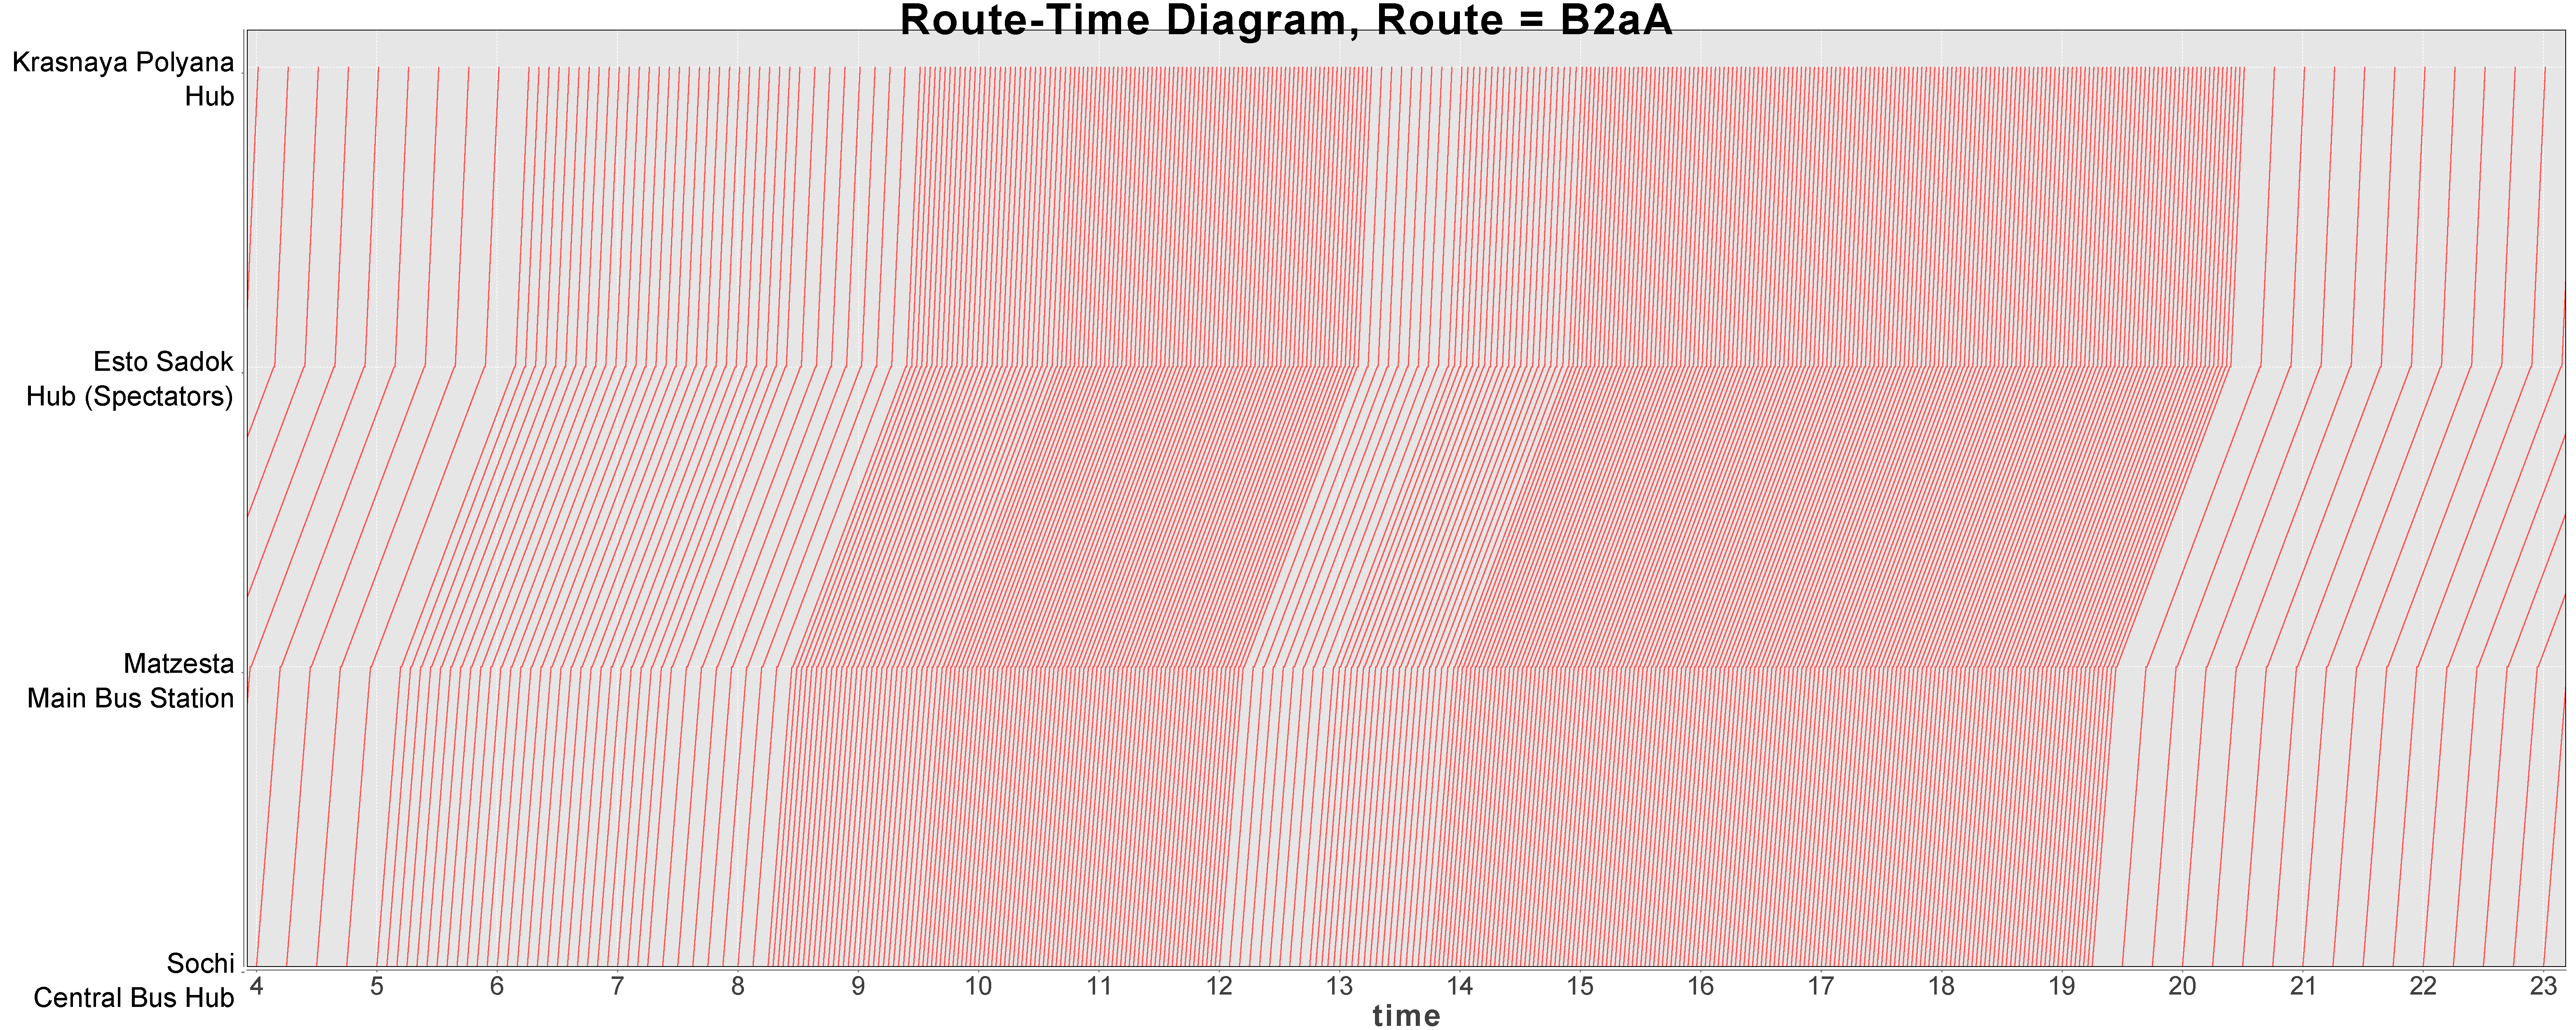
\includegraphics[width=1.\textwidth,angle=0]{./using/figures/sochi_adaptiveSchedule.pdf}}%
{}

In addition to private car traffic and schedule-based public transport, special
transportation offerings typically exist for athlethes, media and officials:
shuttle buses or even limousine services that operate on demand only between two
or more fixed locations. Termed ``transit on demand'' in ITSOS, transit lines
with stops along a route were defined, but without any scheduled departures. 
Instead, a within-day like operator was implemented that scheduled vehicles
whenever an agent of one of the agent groups wanted to depart. The
rule-based operator had additional constraints like a minimum occupancy of
on-demand vehicles before departure (to prevent every on-demand vehicle
transports only a single agent) as well as a maximum waiting time before
departure for such vehicles (to prevent agents on remote locations having to
wait forever).

At sport events, a large number of spectators have to share a few common entries
to event facilities, and share common access paths to those facilities. This
makes it necessary to simulate pedestrian flows at least in certain places in
more detail than just the default teleportation approach typically used by
MATSim. For olympic games, this was even more a requirement due to the fact
that in several locations security checks existed that created additional
bottlenecks. This requirement was solved by implementing a special router for
the walk mode, along with a custom departure handler. The router tries to find a
path on the network for walk legs, taking into account how far the closest walk
link is away from a facility to decide if the link can act as an access to the
facility or not. If no close-by link is found, or not route is found between
two access links, an empty route is stored in the leg. The departure handler
checks if the route is empty or not, either teleporting the agent or putting it
on a walk link in the network. Walk links are regular queue-based network links
with capacity and free-speed set according to the simplified physics of
directed pedestrians flows. This approach made it possible to model the
bottleneck effects of security screening gates easily, as well as consider the
available walk paths available where necessary by modelling them, leaving them
out in other places where it doesn't matter. Figure~\ref{fig:sochi:pedestrians}
shows an example of the simulated pedestrian movements at Krasnaya Polyana, the
area in the mountains near Sochi where a lot of events took place.  
%
\createfigure%
{Simulated Pedestrians at Krasnaya Polyana Hub}%
{Simulated Pedestrians (red circles) at Krasnaya Polyana Hub. Transit vehicles
(incl. cable cars) shown as green boxes, Transit stops as blue circles.}%
{\label{fig:sochi:pedestrians}}%
{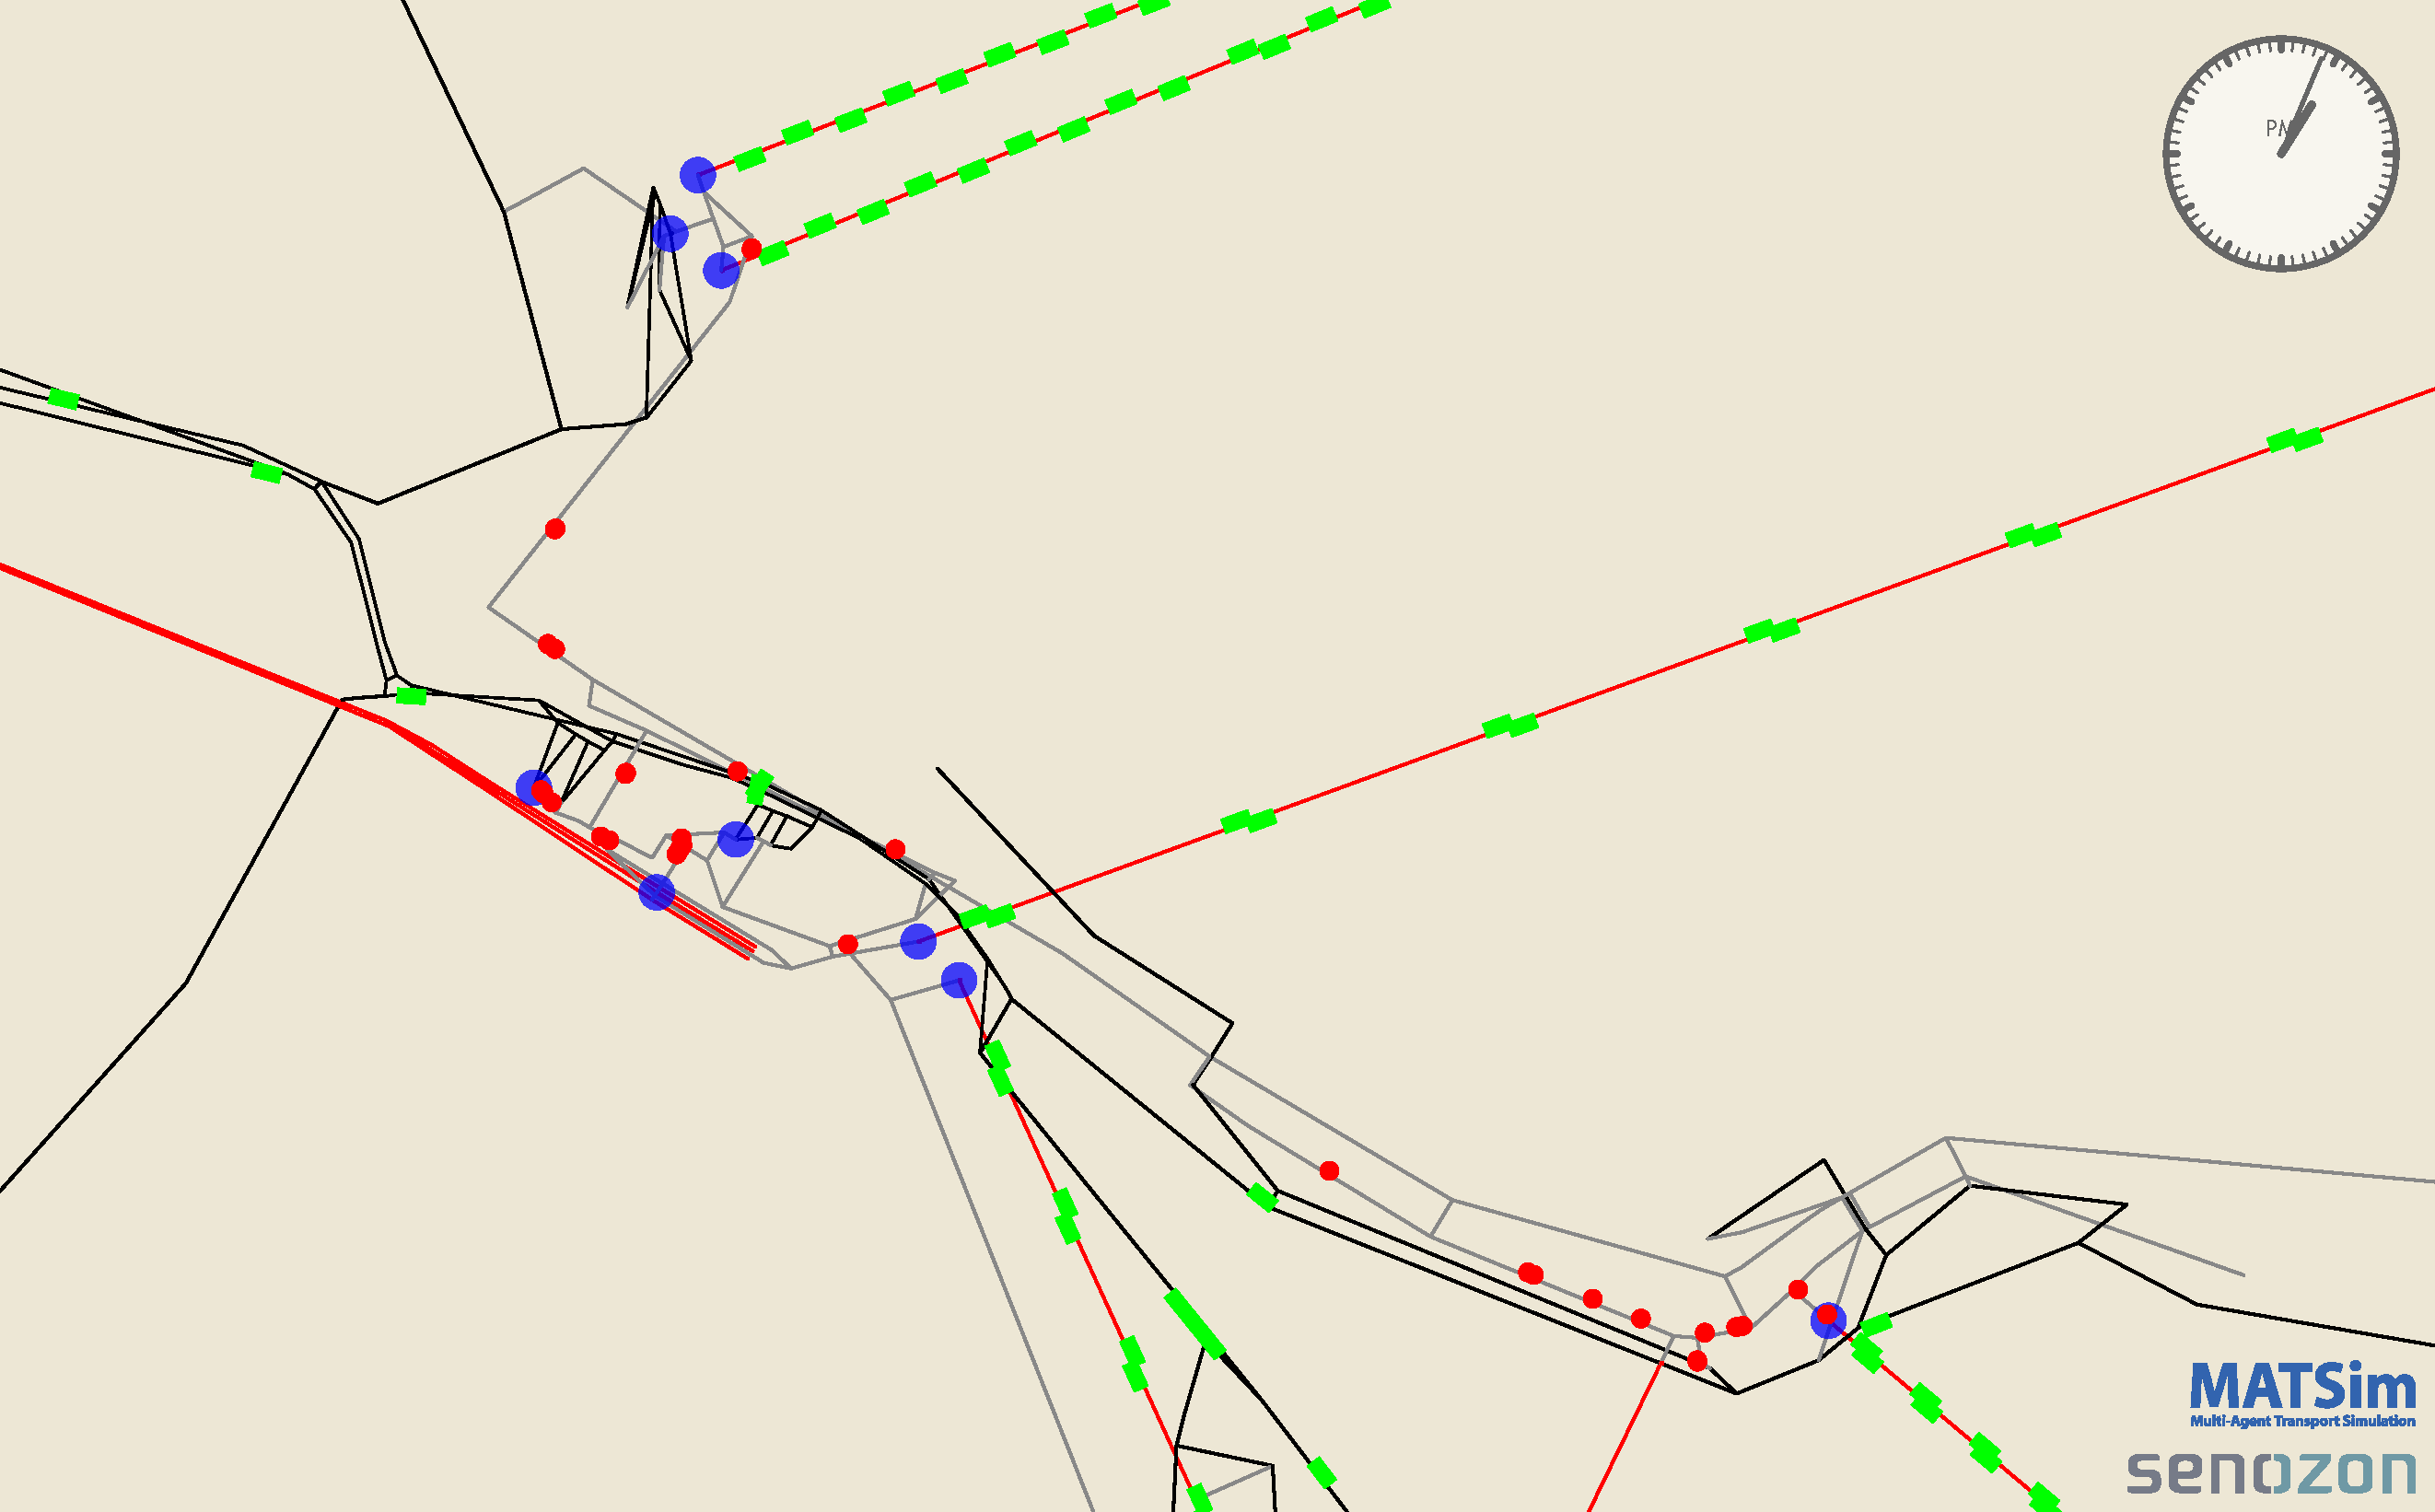
\includegraphics[width=1.\textwidth,angle=0]{./using/figures/sochi_pedestrians.pdf}}%
{}
%

\subsection{Simulation of Sochi}

To test the applicability of ITSOS for transportation planning for major events,
a model of the olympic winter games in Sochi (Russia) 2014 was built. Data was
either collected by workers of Masterconcept or cooperating companies, or
received from Russian governmental institutions.

The road and train network was modelled in ArcGIS using the ITSOS extensions.
The transit schedule included 55 transit lines, a mix of bus lines, train lines,
and cable cars going up into the mountain areas. 24 of those lines were
defined to be adaptive, 19 lines operated on-demand as shuttle services.

Travel demand was
defined for each day of the games, based on the actual schedule of the games,
making assumptions about how many spectators visit each of the different
competitions during the day. While the size of event facilities can be used as a
upper limit for the number of spectators, a lot of expert knowledge available at
Masterconcept was used to define the actual numbers of expected people at each
event.

While events often start and end at different times
of day, due to the fact that many event locations share at least partially a
common route to reach them, an important aspect was to simulate if the offered
transport services are able to cope with the combined travel demand generated
by multiple, separate events.

A typical simulation run of Sochi included about 150~000 agents. To speed up
simulations, parallel events handling and parallel qsim was used. The simulation
generated around 15 million events per iteration.

Figure~\ref{fig:sochi:model} shows a screenshot of the Sochi scenario,
visualized in Via.
%
\createfigure%
{Overview of the Sochi model}%
{Overview of the Sochi model}%
{\label{fig:sochi:model}}%
{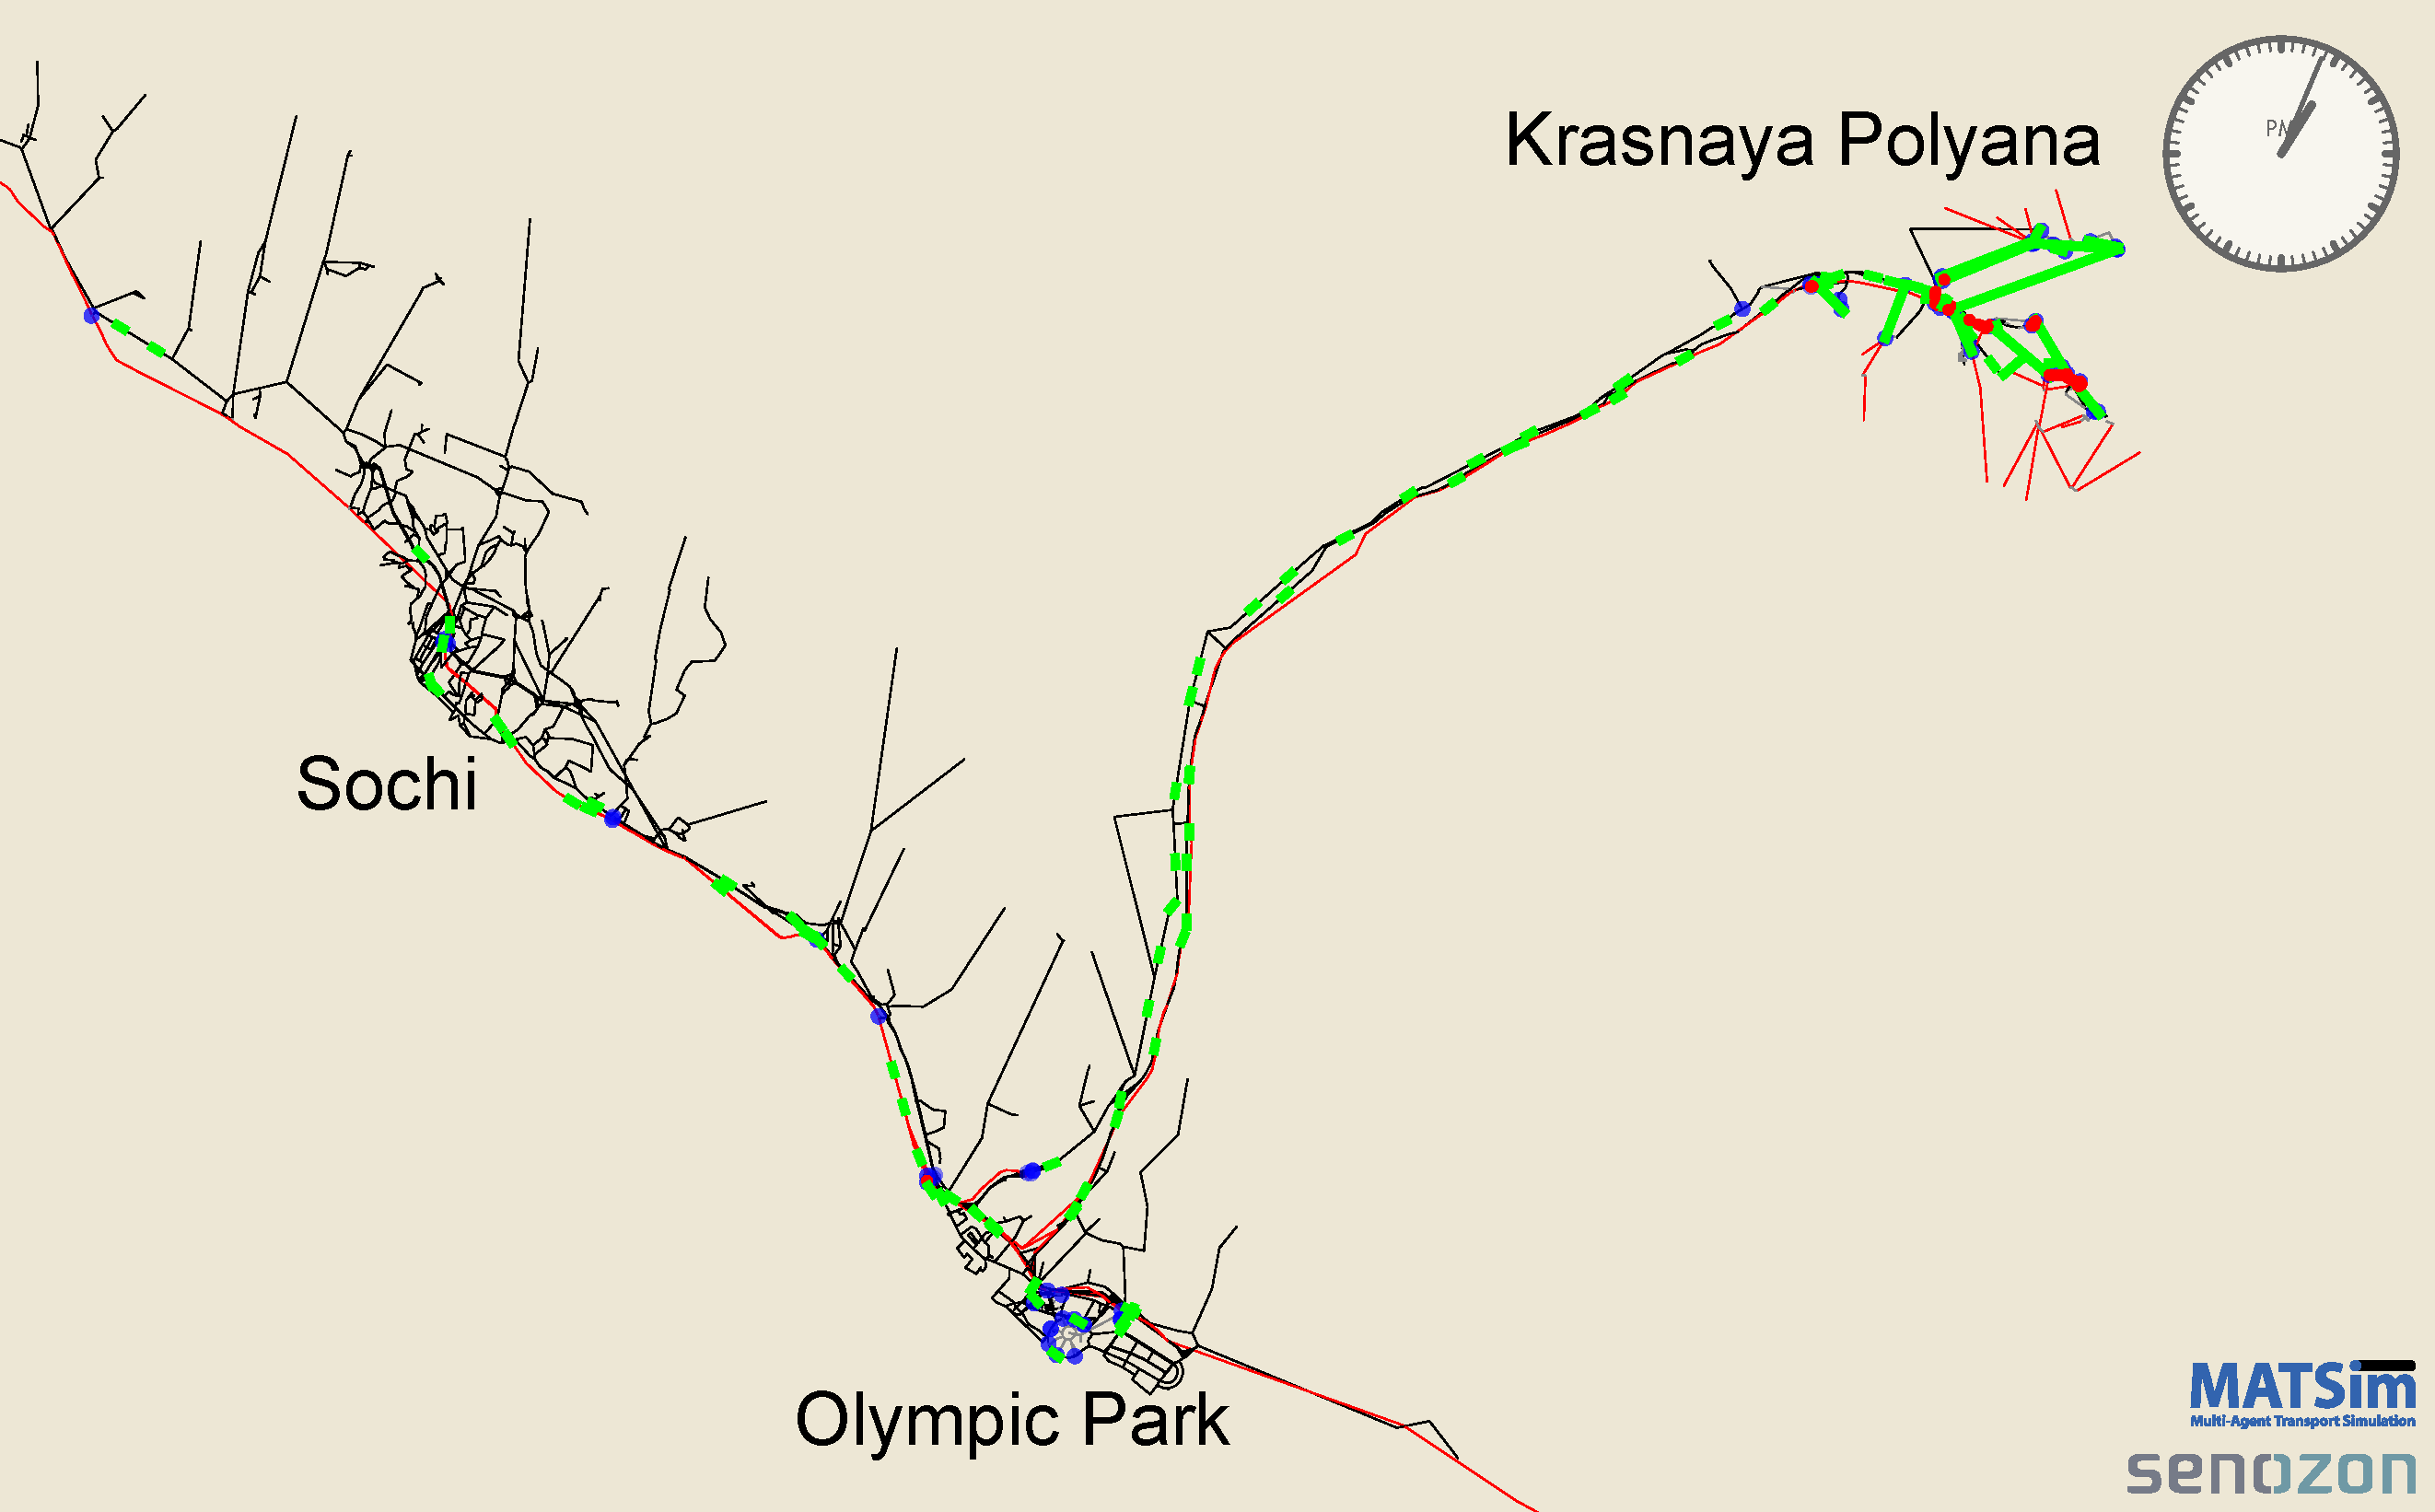
\includegraphics[width=1.\textwidth,angle=0]{./using/figures/sochi_full.pdf}}%
{}
%

\subsection{Outlook}

Besides the test case of the olympic winter games in Sochi in 2014, ITSOS/MATSim
was also used to simulate traffic in St. Johann (Pongau, Austria) with a strong
emphasis on pupils which often need to take a combination of buses and trains to
get to school.

A new company, Masterconcept Mobility GmbH, was split off Masterconcept
Consulting GmbH in 2014 which offers transportation planning services for major
events as well as regional planning services based on the combination of ITSOS
and MATSim.


% ##################################################################################################################